% TriAgent — FinLLM @ IJCAI 2026 submission
% Compile:  pdflatex main && bibtex main && pdflatex main && pdflatex main
% Self-contained: ijcai26.sty + named.bst + figures/*.pdf + sections/*.tex
% all in this directory.

\documentclass{article}
\pdfpagewidth=8.5in
\pdfpageheight=11in

\usepackage{ijcai26}

\usepackage{times}
\usepackage{soul}
\usepackage{url}
\usepackage[hidelinks]{hyperref}
\usepackage[utf8]{inputenc}
\usepackage[small]{caption}
\usepackage{graphicx}
\usepackage{amsmath, amssymb, amsfonts, amsthm}
\usepackage{booktabs}
\usepackage{multirow}
\usepackage{algorithm}
\usepackage{algpseudocode}
\usepackage[switch]{lineno}

% Line numbers disabled (FinLLM/IJCAI 2026 submission does not require lineno)
% \linenumbers

\urlstyle{same}

\graphicspath{{figures/}}

\pdfinfo{
/TemplateVersion (IJCAI.2026.0)
}

\title{TriAgent: Divergence-Aware Multi-Agent Committees for
       Cost-Efficient and Privacy-Preserving Financial Sentiment Analysis}

\author{
Isabel Xu$^{1,*}$
\and
Cynthia Xu$^{1,*}$\and
Rachel Ren$^2$\and
Cong Guo$^3$\and
Jiacheng Ding$^{3,\dagger}$\\
\affiliations
$^1$The Overlake School\\
$^2$Edwards Vacuum Inc.\\
$^3$The University of Memphis\\
\emails
\{xushuyao, xuningshu\}@gmail.com,
rachelren@gmail.com,
\{cguo, jding2\}@memphis.edu\\
$^*$Equal contribution. \quad $^\dagger$Corresponding author.
}

\begin{document}
\maketitle

\begin{abstract}
Production deployments of LLM-based financial sentiment analysis face
a structural cost problem: most queries are trivially classifiable yet
are routinely processed by expensive cloud reasoners, and the bill
scales linearly with user count.
We present \textbf{TriAgent}, a divergence-aware multi-agent committee
that stacks three increasingly contextual tiers --- a word-level
lexicon agent (VADER), a sentence-level domain transformer (FinBERT),
and a cross-sentence reasoner (Qwen2.5-Instruct, swept from 0.5\,B to
14\,B-4bit and across families) --- and routes queries by a three-way
\emph{Semantic Divergence Index} (SDI). On Financial PhraseBank we
find: (i) the domain specialist alone (F1$=$0.88) outperforms every
generic LLM up to 7\,B (F1$=$0.81) at $60\times$ lower cost; (ii) when
the LLM is re-tasked as a \emph{critic} over the smaller agents'
outputs, F1 plateaus at $\approx$0.87 across model sizes from 1.5\,B
to 7\,B --- ``\emph{interaction substitutes for parameters}'' --- but
this plateau is granularity-stratified, not multi-agent-per-se: a
3-persona Qwen-1.5B vote drops to F1$=$0.66; (iii) a Shared Consensus
Dictionary (SCD) using multilingual sentence-BERT serves as a
cross-lingual canonicalizer, answering 95\% of Chinese queries from an
English cache at F1$=$0.99; (iv) the same SDI signal that gates
routing doubles as a post-hoc LLM-hallucination detector at AUC$=$0.90.
A 20-ticker backtest shows the SDI two-stage strategy attains the best
risk-adjusted return (Sharpe$=$3.50) among all evaluated strategies,
and a scale analysis shows TriAgent saves \$9.3\,M/year vs. the
default-to-cloud-LLM baseline at 10\,M users. The framework is
fully open-source and edge-deployable on a single 24\,GB GPU.
\end{abstract}

\section{Introduction}
\label{sec:intro}

A mid-sized asset manager with 1\,M users running 10 sentiment
queries each per trading day generates $\sim$3.6\,B inference calls
per year. At the public price of GPT-4o-mini that single workload
costs $\sim$\$1.1\,M/year; at GPT-4 prices, $\sim$\$36.5\,M/year
(Figure~\ref{fig:cost}). The cost scales linearly with user count
while the value of each LLM call falls --- most domain queries are
trivially classifiable. \textbf{Token efficiency} --- spending fewer
tokens per query, on cheaper agents, with fewer escalations --- is
therefore the first-order operational concern, not an afterthought.
The CFP for FinLLM@IJCAI 2026 calls out exactly this regime:
multi-agent cloud-edge collaboration, token economics, and
cross-border fairness in deployment.

\begin{figure}[t]
\centering
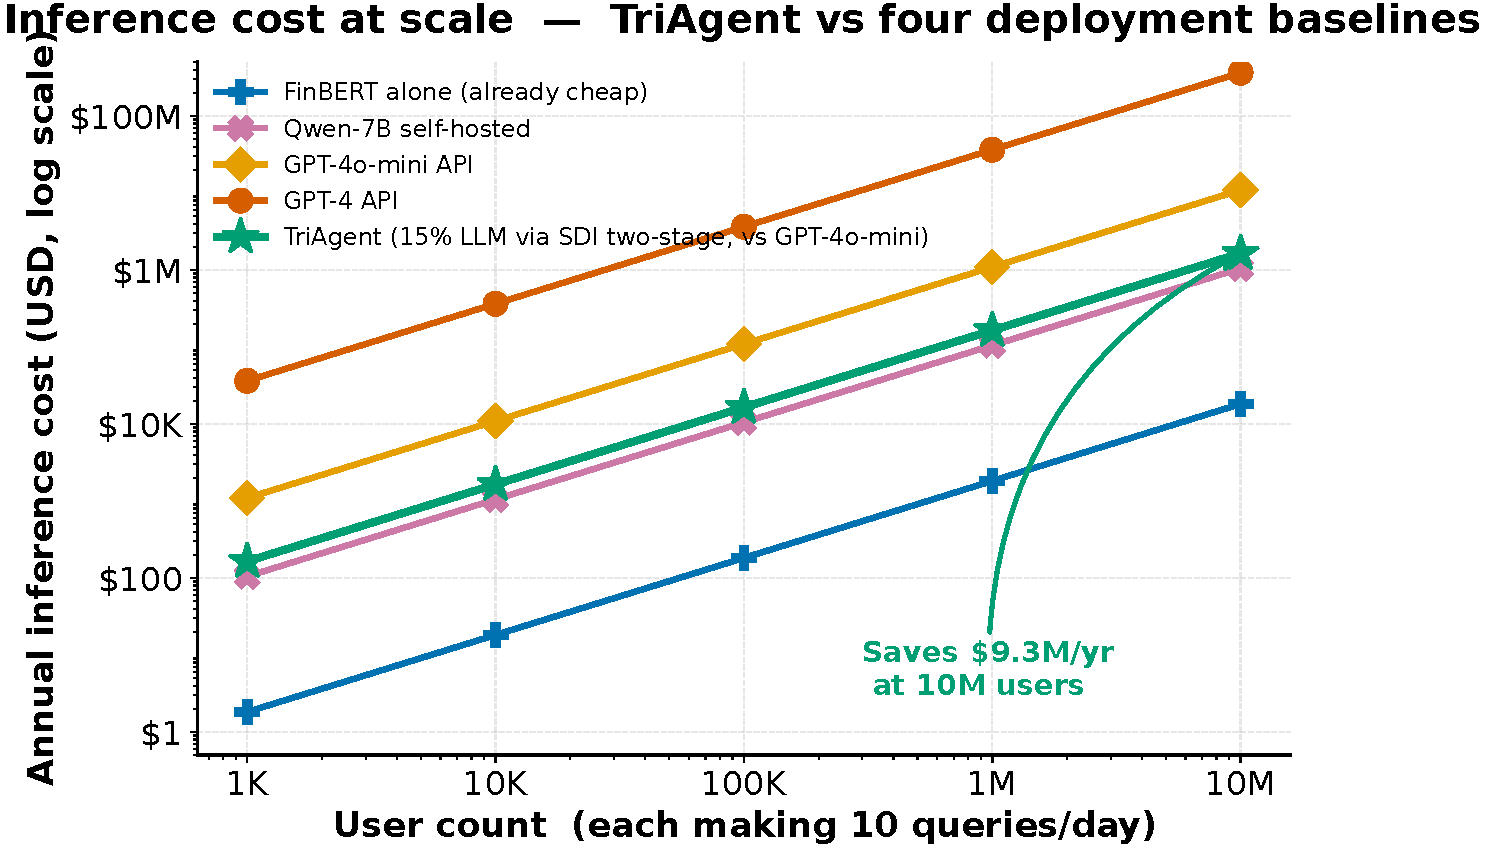
\includegraphics[width=\columnwidth]{fig_cost_at_scale.pdf}
\caption{Annual inference cost vs.\ user count (10 queries/user/day).
At 10\,M users, default-to-cloud-LLM costs \$11\,M--\$365\,M/yr;
TriAgent shaves this to \$1.65\,M/yr, a \$9.3\,M/yr saving against
GPT-4o-mini.}
\label{fig:cost}
\end{figure}

\paragraph{Running example.}
Throughout we trace one FPB sentence:
\textit{``\dots its net profit halved to 1.2~mln euro\dots from
2.2~mln euro\dots''} (gold $=$ negative).
VADER ($+0.44$) and FinBERT ($+0.53$) are both fooled by the surface
word \emph{profit}; Qwen-7B alone correctly outputs negative
($-0.80$, ``profit declined''); critic@1.5B and critic@7B are
\emph{anchored} on V$+$F's positives and stay wrong; only round-2
debate, which feeds back the LLM's own R1 rationale, recovers
negative. This single example threads through
Sections~\ref{sec:framework}--\ref{sec:security}.

\paragraph{Contributions.}
\textsc{TriAgent} is a divergence-aware committee whose three tiers
correspond to three contextual granularities (word $\to$ sentence
$\to$ cross-sentence). We contribute:
\textbf{(C1)} a three-way Semantic Divergence Index (SDI) with a
four-quadrant routing interpretation;
\textbf{(C2)} the \emph{critic plateau} --- critic@1.5B$/$3B$/$7B
all reach F1$=$0.87, while a same-size 3-persona vote regresses to
F1$=$0.66, identifying granularity-stratified diversity (not
multi-agent voting per se) as the mechanism;
\textbf{(C3)} a Shared Consensus Dictionary (SCD) over multilingual
sentence embeddings that doubles as a cross-lingual canonicaliser
(95\% of Chinese queries match an English cached label at
F1$=$0.99);
\textbf{(C4)} a three-granularity edge predictor (XGBoost AUC$=$0.85)
enabling fully on-device routing;
\textbf{(C5)} an empirical security side-benefit --- the same SDI
acts as a post-hoc LLM-hallucination flag at AUC$=$0.90;
\textbf{(C6)} a 20-ticker back-test where the SDI single-stage
strategy attains the best Sharpe ($3.50$) of all evaluated
strategies, including always-FinBERT ($1.36$) and always-LLM
($0.11$).
A single architectural decision --- small agents stratified by
granularity, plus an SDI gate, plus an embedding cache --- hits all
three FinLLM 2026 CFP topic buckets simultaneously.

\section{Related Work}
\label{sec:related}

\paragraph{Financial NLP.}
Loughran and McDonald~\shortcite{loughran2011liability} flagged
systematic miscalibration of generic sentiment lexicons in financial
text; Financial PhraseBank~\cite{malo2014fpb} grew out of that line.
FinBERT~\cite{araci2019finbert,yang2020finbert} is the de facto open
domain transformer; surveys~\cite{wang2024finllmsurvey} document a
recent wave of billion-parameter financial reasoners
(BloombergGPT~\cite{wu2023bloomberggpt},
FinGPT~\cite{yang2023fingpt}, PIXIU~\cite{xie2023pixiu}). We ask
\emph{not} which model is best, but how small each agent in a
committee can become.

\paragraph{Multi-agent LLMs.}
Query-by-committee~\cite{settles2009al} and ensemble
disagreement~\cite{lakshminarayanan2017ensembles} are the classical
ancestors of our SDI. Recent multi-agent LLM frameworks ---
AutoGen~\cite{wu2023autogen}, MetaGPT~\cite{hong2023metagpt},
CAMEL~\cite{li2023camel}, multi-agent
debate~\cite{du2023debate,liang2023encouraging}, LLM-as-a-judge
\cite{zheng2023judging}, self-consistency
\cite{wang2023selfconsistency} --- typically use the \emph{same}
large model for every agent. Our negative result on same-size
persona vote (Section~\ref{sec:experiments:scaling}) shows this does
not substitute for the granularity-stratified diversity that drives
our critic plateau.

\paragraph{Cost-aware routing and semantic caching.}
FrugalGPT~\cite{chen2023frugalgpt}, RouteLLM~\cite{ong2024routellm},
and mixture-of-models routing~\cite{wang2022mixture,shnitzer2023llmrouting}
cascade between cheap and expensive models per query. Semantic
caches~\cite{wang2024caching} (a sibling of our SCD) reduce inference
cost by reusing answers for near-duplicate queries; our SCD differs
in that it caches \emph{committee decisions} (not single-model
outputs) and uses multilingual sentence
embeddings~\cite{reimers2019sbert,reimers2020multilingualkd} for
cross-lingual canonicalisation.

\section{Framework}
\label{sec:framework}

\begin{figure}[t]
\centering

\includegraphics[width=0.95\columnwidth]{fig_architecture.pdf}
\caption{TriAgent system architecture. A query first hits the SCD;
on cache miss the three-tier committee runs
(VADER$\to$FinBERT$\to$Qwen-$N$), then SDI computation, then an
interaction protocol when SDI exceeds threshold. The final
committee label is written back into the SCD.}
\label{fig:architecture}
\end{figure}

\subsection{Three-Tier Committee as a Granularity Stack}
\label{sec:framework:committee}

Figure~\ref{fig:architecture} sketches the system end-to-end. The
three tiers correspond to three contextual granularities:
\textbf{L1 VADER}~\cite{hutto2014vader} (word-level lexicon,
$\approx$0.03\,ms);
\textbf{L2 FinBERT}~\cite{araci2019finbert} (sentence-level
transformer, 110\,M params, $\approx$1.5\,ms);
\textbf{L3 Qwen2.5-Instruct-$N$}~\cite{qwen25} (cross-sentence
reasoner; $N\!\in\!\{0.5,1.5,3,7,14\text{-4bit}\}$\,B, plus
cross-family Mistral-7B~\cite{mistral7b}). VADER fails on
phrase-bound polarity reversals (\textit{loss narrowed}); FinBERT
fails on multi-clause numeric comparisons; the LLM over-confidently
invents reasoning where lexicon neutrality is correct. Pairwise
error-set Jaccard between the three is only $0.13$--$0.15$
(Section~\ref{sec:experiments:bias}) --- the empirical signature of
granularity-orthogonal failures.

\paragraph{Deployment-style example.}
Consider an Apple-style news sentence routed at runtime:
\textit{``services revenue grew but iPhone unit volumes declined
sharply against a difficult comparable.''} VADER's lexicon picks up
\emph{grew} and outputs positive ($+0.31$); FinBERT, attending only
within the sentence, returns weakly negative ($-0.18$); Qwen-7B
correctly outputs strongly negative ($-0.62$) by reasoning across
clauses. SDI$_{\mathrm{ER}}$ exceeds threshold and the SDI gate
fires the critic protocol, which returns the LLM's label as final.
This is the routing behaviour the architecture is designed to
exhibit; the same mechanism applied to the running FPB sentence in
Section~\ref{sec:intro} is the empirical anchor used throughout the
paper.

\subsection{Three-Way Semantic Divergence Index}
\label{sec:framework:sdi}

Let $s_{\mathrm{V}}, s_{\mathrm{F}}, s_{\mathrm{L}} \in [-1, +1]$
denote the continuous polarity scores emitted by V, F, L
respectively. We define three pairwise Semantic Divergence Indices,
one per granularity-pair:
\begin{equation}
\label{eq:sdi}
\begin{aligned}
\mathrm{SDI}_{\mathrm{LE}} &= |s_{\mathrm{V}} - s_{\mathrm{F}}|,
\quad
\mathrm{SDI}_{\mathrm{LR}}  = |s_{\mathrm{V}} - s_{\mathrm{L}}|,\\
\mathrm{SDI}_{\mathrm{ER}} &= |s_{\mathrm{F}} - s_{\mathrm{L}}|.
\end{aligned}
\end{equation}
Each $\mathrm{SDI}\in [0,2]$ measures the disagreement between two
agents operating at \emph{different} granularities. We additionally
track $\mathrm{SDI}_{\max}=\max(\mathrm{SDI}_{\mathrm{LE}},
\mathrm{SDI}_{\mathrm{LR}},\mathrm{SDI}_{\mathrm{ER}})$ and
$\overline{\mathrm{SDI}}$ (mean). Thresholding the pair
$(\mathrm{SDI}_{\mathrm{LE}},\mathrm{SDI}_{\mathrm{ER}})$ at
$(\tau_{\mathrm{LE}},\tau_{\mathrm{ER}})=(0.3,0.7)$ partitions
samples into four behaviour \emph{quadrants}:
\begin{equation}
\label{eq:quadrant}
Q(x) = \begin{cases}
\textit{consensus}     & \mathrm{SDI}_{\mathrm{LE}} \le 0.3 \land \mathrm{SDI}_{\mathrm{ER}} \le 0.7 \\
\textit{domain shift}  & \mathrm{SDI}_{\mathrm{LE}} >    0.3 \land \mathrm{SDI}_{\mathrm{ER}} \le 0.7 \\
\textit{ambiguous}     & \mathrm{SDI}_{\mathrm{LE}} \le 0.3 \land \mathrm{SDI}_{\mathrm{ER}} >    0.7 \\
\textit{mixed}         & \text{otherwise}.
\end{cases}
\end{equation}
Each quadrant carries a distinct downstream implication
(Table~\ref{tab:quadrant}): consensus skips L3, domain shift trusts
F and routes around V, ambiguous fires the LLM critic, and mixed
escalates to debate.

\subsection{Routing and Interaction Protocols}
\label{sec:framework:routing}

Routing strategies S0--S2 are the three single-agent baselines;
S3--S5 escalate L1$\to$L2 by random / confidence /
SDI$_{\mathrm{LE}}$; S6 is a two-stage cascade adding L2$\to$L3 by
SDI$_{\mathrm{ER}}$. Formally, the two-stage routing decision at a
sentence $x$ is
\begin{equation}
\label{eq:routing}
\hat{y}(x) =
\begin{cases}
\mathcal{I}(x; V, F, L) & \mathrm{SDI}_{\mathrm{ER}}(x) > \theta_{\mathrm{ER}} \\
F(x)                    & \mathrm{SDI}_{\mathrm{LE}}(x) > \theta_{\mathrm{LE}} \\
V(x)                    & \text{otherwise,}
\end{cases}
\end{equation}
where $\mathcal{I}\in\{\text{vote}, \text{critic}, \text{debate}\}$
is the interaction protocol. \textbf{Vote} returns the
confidence-weighted majority over V/F/L; \textbf{critic} feeds the
LLM the original sentence plus V's and F's predictions and asks for
a final label; \textbf{debate} performs a round-2 LLM call that sees
all three round-1 outputs (including its own rationale) and
reconciles. The thresholds $(\theta_{\mathrm{LE}},
\theta_{\mathrm{ER}})$ sweep out the Pareto frontier of
Section~\ref{sec:experiments:pareto}.

Algorithm~\ref{alg:triagent} summarises the end-to-end inference
flow including the SCD cache.

\begin{algorithm}[t]
\caption{TriAgent inference (single query)}
\label{alg:triagent}
\begin{algorithmic}[1]
\Require query $x$; thresholds $\tau, \theta_{\mathrm{LE}}, \theta_{\mathrm{ER}}$;
agents $V, F, L$; interaction $\mathcal{I}$; SCD cache $\mathcal{C}$
\Ensure label $\hat{y}$
\State $(\tilde{x}, \sigma) \gets$ nearest-neighbour in $\mathcal{C}$ by cosine
\If{$\sigma \ge \tau$}
  \State \Return $\mathcal{C}[\tilde{x}]$ \Comment{cache hit, no model call}
\EndIf
\State $s_{\mathrm{V}} \gets V(x)$; $\;s_{\mathrm{F}} \gets F(x)$
\State compute $\mathrm{SDI}_{\mathrm{LE}}=|s_{\mathrm{V}}-s_{\mathrm{F}}|$
\If{$\mathrm{SDI}_{\mathrm{LE}} \le \theta_{\mathrm{LE}}$}
  \State $\hat{y} \gets V(x)$ \Comment{lexicon suffices}
\Else
  \State $s_{\mathrm{L}} \gets L(x)$
  \State compute $\mathrm{SDI}_{\mathrm{ER}}=|s_{\mathrm{F}}-s_{\mathrm{L}}|$
  \If{$\mathrm{SDI}_{\mathrm{ER}} > \theta_{\mathrm{ER}}$}
    \State $\hat{y} \gets \mathcal{I}(x; s_{\mathrm{V}}, s_{\mathrm{F}}, s_{\mathrm{L}})$
  \Else
    \State $\hat{y} \gets F(x)$
  \EndIf
\EndIf
\State $\mathcal{C}.\textsc{Put}(x, \hat{y})$
\Comment{populate cache for future queries}
\State \Return $\hat{y}$
\end{algorithmic}
\end{algorithm}

\subsection{Shared Consensus Dictionary}
\label{sec:framework:scd}

An optional fourth component caches committee decisions in
multilingual sentence-BERT embedding
space~\cite{reimers2019sbert,reimers2020multilingualkd}. Let
$\phi(\cdot)\in\mathbb{R}^{384}$ denote the sentence-BERT encoder. A
query $x$ is embedded to $\phi(x)$, $k$-NN-searched against cached
entries $\{(\tilde{x}_i, y_i)\}$ by cosine similarity
$\sigma_i = \langle\phi(x),\phi(\tilde{x}_i)\rangle / (\|\phi(x)\|\|\phi(\tilde{x}_i)\|)$,
and the cached label is returned when
\begin{equation}
\label{eq:scdrule}
\sigma^{\ast}(x) = \max_{i} \sigma_i \;\ge\; \tau,
\end{equation}
i.e.\ \emph{without any model call}. The SCD is sentence-granularity
by construction --- \emph{``net profit halved''} matches
\emph{``net profit cut in half''} which exact-match memoisation
would miss. Threshold $\tau$ is a single operator knob trading hit
rate against accuracy (Section~\ref{sec:experiments:scd}). Beyond
cost, the SCD supplies cross-committee consistency: a new agent that
joins the committee inherits the cache, mitigating the
family-specific plateau gap we observe with Mistral-7B
(Section~\ref{sec:experiments:scaling}).

\section{Three-Granularity Edge Predictor}
\label{sec:predictor}

For routing to be deployable, the gating decision must be made
\emph{before} any expensive model has run. We train a lightweight
classifier to predict, from features computable at the VADER stage
alone, whether a sentence will produce high committee disagreement
(binary target: $\mathrm{SDI}_{\max}>0.7$). The feature engineering
mirrors the committee's own granularity stratification ---
word, phrase, and sentence --- and we report the marginal
contribution of each.

\paragraph{Word-level.}
6 VADER outputs (positive/negative/neutral fractions, compound,
confidence, $|$compound$|$) and 6 surface indicators (number,
currency, contrast word, negation, length). We mine \emph{unigram}
triggers via log-odds + $z$-score on the high-SDI subset; top words
include \texttt{decreased}, \texttt{dropped}, \texttt{fell}.

\paragraph{Phrase-level.}
We extend the log-odds miner to $n\!\in\!\{2,3\}$ and use the
top-30 bigram / trigram triggers as binary presence features.
Bigrams capture phrase-bound polarity that single words miss
(\texttt{down\_from}, \texttt{compared\_profit}, and ideally
context-flipping pairs like \texttt{loss\_narrowed} vs.\
\texttt{loss\_widened}). On FPB the bigram lift is small ($+0.01$
AUC over unigram), but the running example
(Section~\ref{sec:intro}) shows the linguistic mechanism is real.

\paragraph{Sentence-level.}
We encode each sentence with the multilingual MiniLM-L12 model
(22\,M params, $\approx$10\,ms/sentence on CPU) and PCA-reduce the
384-dim embedding to 16 components. The same module powers the SCD
(Section~\ref{sec:framework:scd}) and the cross-lingual pilot
(Section~\ref{sec:experiments:zh}).

Table~\ref{tab:predictor} reports the seven-variant ablation. Word
features alone reach AUC $=0.69$; phrase adds $+0.01$;
\emph{sentence} adds $+0.04$ --- the largest single-granularity
contribution. XGBoost over the full feature set reaches AUC $=0.85$.
A non-deployable upper bound that encodes the LLM's R1 reasoning
text reaches AUC $=0.94$, marking remaining headroom for deployable
variants.

\begin{table*}[t]
\centering
\small
\caption{Edge predictor ablation across the three feature
granularities. AUC-PR = area under precision-recall;
P@R$x$ = precision at $x$\,\% recall; P@top10 = precision among the
10\,\% riskiest predictions. Sentence-BERT features add the largest
single-granularity lift. The non-deployable upper bound encodes the
LLM's R1 explanation text and is not counted toward the deployable
ceiling.}
\label{tab:predictor}
\begin{tabular}{lrrrrr}
\toprule
Model & AUC-ROC & AUC-PR & P@R20 & P@R50 & P@top10 \\
\midrule
random              & 0.503 & 0.328 & 0.353 & 0.332 & 0.351 \\
LR-unigram          & 0.694 & 0.566 & 0.788 & 0.479 & 0.773 \\
LR-uni+bigram       & 0.697 & 0.570 & 0.764 & 0.486 & 0.742 \\
LR-uni+bi+trigram   & 0.703 & 0.582 & 0.808 & 0.503 & 0.773 \\
LR-sentence-only    & 0.688 & 0.583 & 0.944 & 0.472 & 0.814 \\
\textbf{LR-uni+bi+sent.} & \textbf{0.741} & \textbf{0.607} & 0.768 & 0.554 & 0.742 \\
\textbf{XGBoost (all)}   & \textbf{0.848} & \textbf{0.745} & \textbf{0.943} & \textbf{0.759} & \textbf{0.866} \\
\midrule
XGBoost+reasoning$^\dagger$ & 0.937 & 0.897 & 0.990 & 0.964 & 0.990 \\
\bottomrule
\end{tabular}
\\[2pt]
\footnotesize $^\dagger$Encodes the LLM's R1 explanation text
(non-deployable upper bound).
\end{table*}

\section{Experiments}
\label{sec:experiments}

\paragraph{Setup.}
We use the \texttt{sentences\_allagree} subset of Financial
PhraseBank~\cite{malo2014fpb,flarefpb} (4{,}838 unique sentences after
deduplication: 604 negative, 2{,}872 neutral, 1{,}362 positive).
LLM inference uses HuggingFace Transformers~\cite{wolf2020transformers}
in bf16 (4-bit for 14\,B via bitsandbytes~\cite{dettmers2023bnb}) on
a single NVIDIA RTX A5000 (24\,GB), batch size 8, deterministic
decoding. Cost is reported in USD using GPU-rental amortisation
(\$0.40/hour A5000-class) for FinBERT and Qwen; VADER cost is
$\approx\!0$. All experiments are reproducible from
\texttt{experiments/L*.py}.

\subsection{Bias Diversity and Four Quadrants}
\label{sec:experiments:bias}

Table~\ref{tab:quadrant} reports the four-quadrant decomposition of
the committee on FPB; Figure~\ref{fig:sdi} visualises the underlying
SDI distributions and class-conditional separation.

\begin{table*}[t]
\centering
\small
\caption{Four quadrants of committee behaviour. The negative class
concentrates in \textit{domain shift} (where VADER fails badly);
ambiguous cases are where the LLM and FinBERT disagree most. $n$
is sample count; Acc$_\mathrm{V/F/L}$ is per-agent accuracy in that
quadrant.}
\label{tab:quadrant}
\begin{tabular}{lrrrrrrrr}
\toprule
Quadrant & $n$ & \% & \%pos & \%neu & \%neg
         & Acc$_\mathrm{V}$ & Acc$_\mathrm{F}$ & Acc$_\mathrm{L}$ \\
\midrule
consensus     & 1907 & 39.4 & 10.7 & 88.7 &  0.5 & 74.6 & 96.4 & 96.5 \\
mixed         & 1509 & 31.2 & 34.1 & 56.9 &  9.0 & 47.2 & 86.0 & 87.2 \\
domain shift  &  651 & 13.5 & 34.6 & 10.1 & 55.3 & 10.3 & 95.5 & 95.5 \\
ambiguous     &  771 & 15.9 & 54.2 & 33.1 & 12.7 & 55.6 & 70.8 & 28.1 \\
\bottomrule
\end{tabular}
\end{table*}

\begin{figure*}[t]
\centering
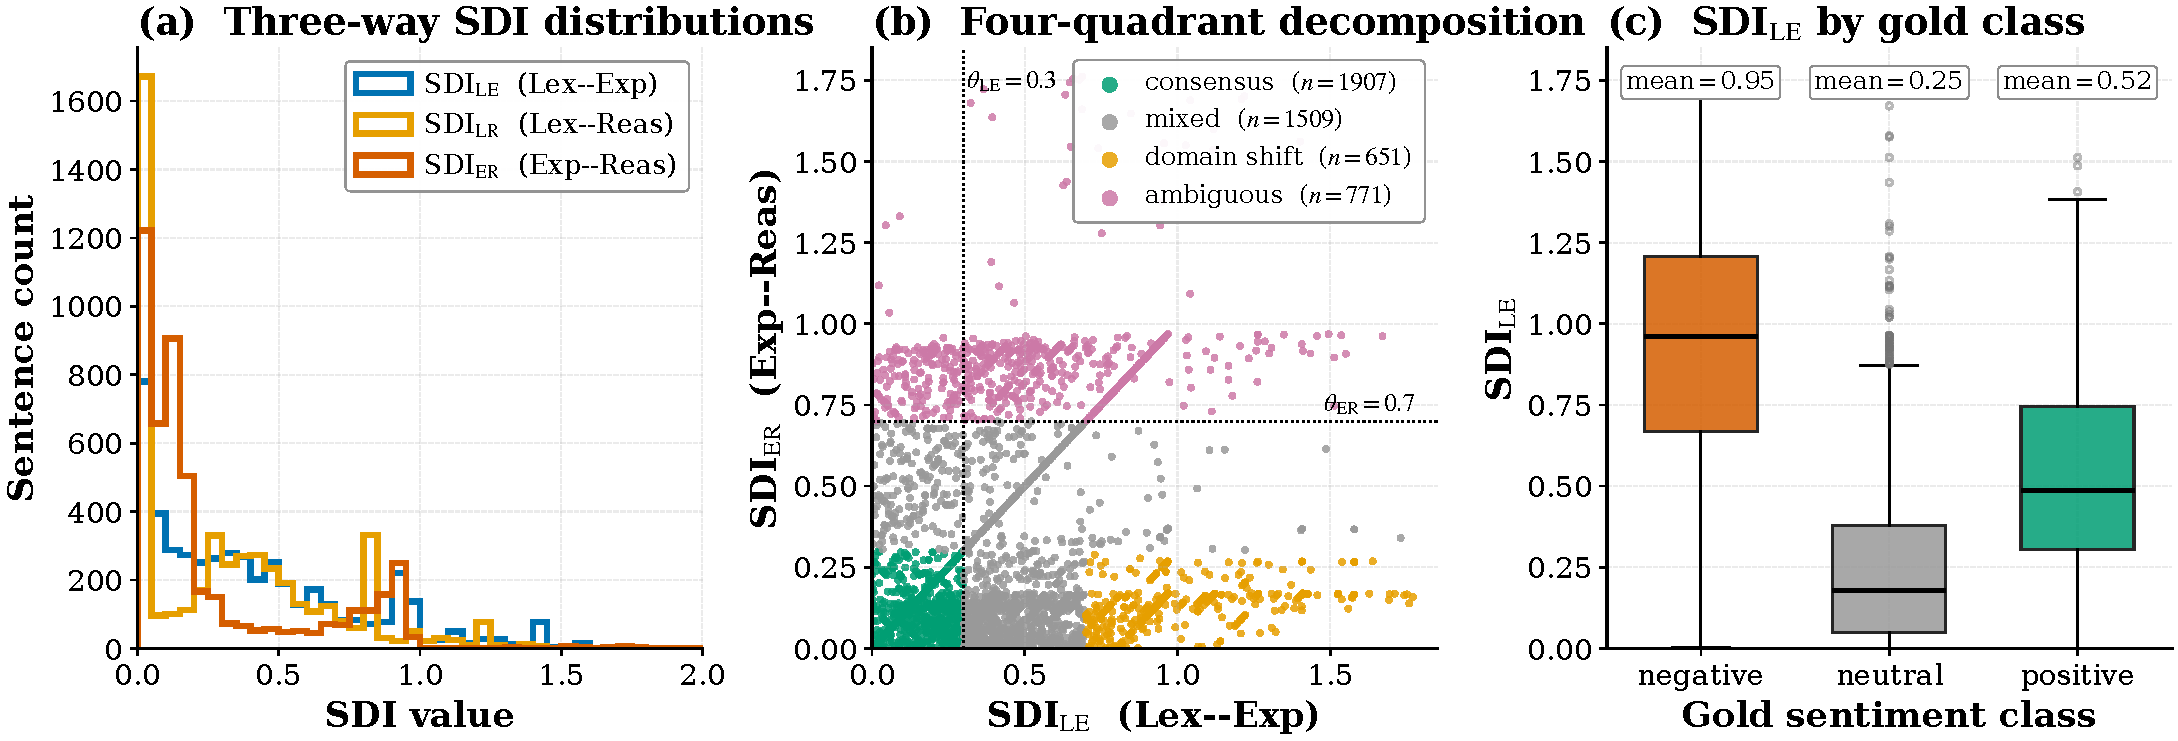
\includegraphics[width=0.9\textwidth]{fig_sdi_three_way.pdf}
\caption{Three-way SDI on FPB. \emph{Left:} distributions of the
three pairwise SDIs. \emph{Centre:} four-quadrant scatter of
$(\mathrm{SDI}_{\mathrm{LE}}, \mathrm{SDI}_{\mathrm{ER}})$.
\emph{Right:} SDI$_{\mathrm{LE}}$ by gold class --- negative has
highest mean disagreement (0.945; ANOVA $F=1777$, $p<10^{-200}$).}
\label{fig:sdi}
\end{figure*}

Pairwise Cohen's $\kappa$ between agent labels (Figure~\ref{fig:bias})
is low: $\kappa(\mathrm{V},\mathrm{F})=0.27$,
$\kappa(\mathrm{F},\mathrm{L})=0.61$,
$\kappa(\mathrm{V},\mathrm{L})=0.19$. Single-agent error sets are
nearly orthogonal --- pairwise Jaccard overlap $0.13$--$0.15$ ---
which is what makes the committee genuinely complementary rather
than a redundant ensemble.

\begin{figure}[t]
\centering
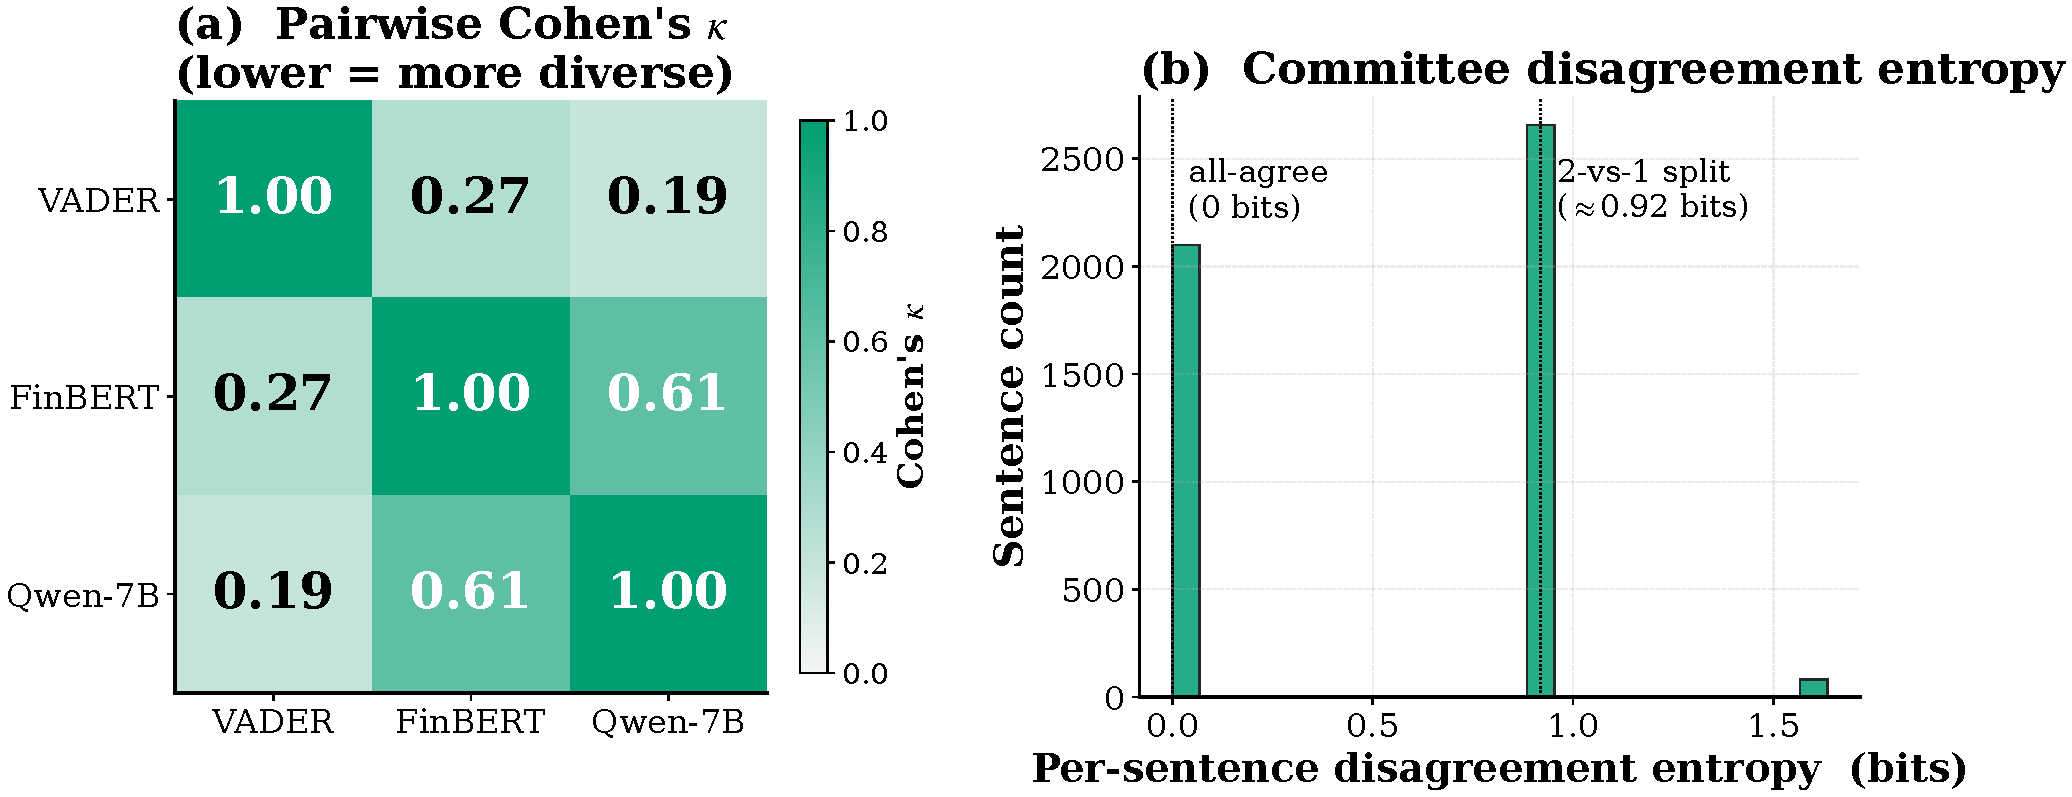
\includegraphics[width=\columnwidth]{fig_bias_diversity.pdf}
\caption{Pairwise Cohen's $\kappa$ (left) and per-sample
disagreement entropy (right). Low $\kappa$ confirms bias diversity;
the bimodal entropy distribution shows the committee is either
fully aligned or split 2-vs-1.}
\label{fig:bias}
\end{figure}

\subsection{Single-Agent Scaling and Critic Plateau}
\label{sec:experiments:scaling}

Figure~\ref{fig:scaling} reports single-agent F1 across the
Qwen2.5-Instruct family.

\begin{figure}[t]
\centering
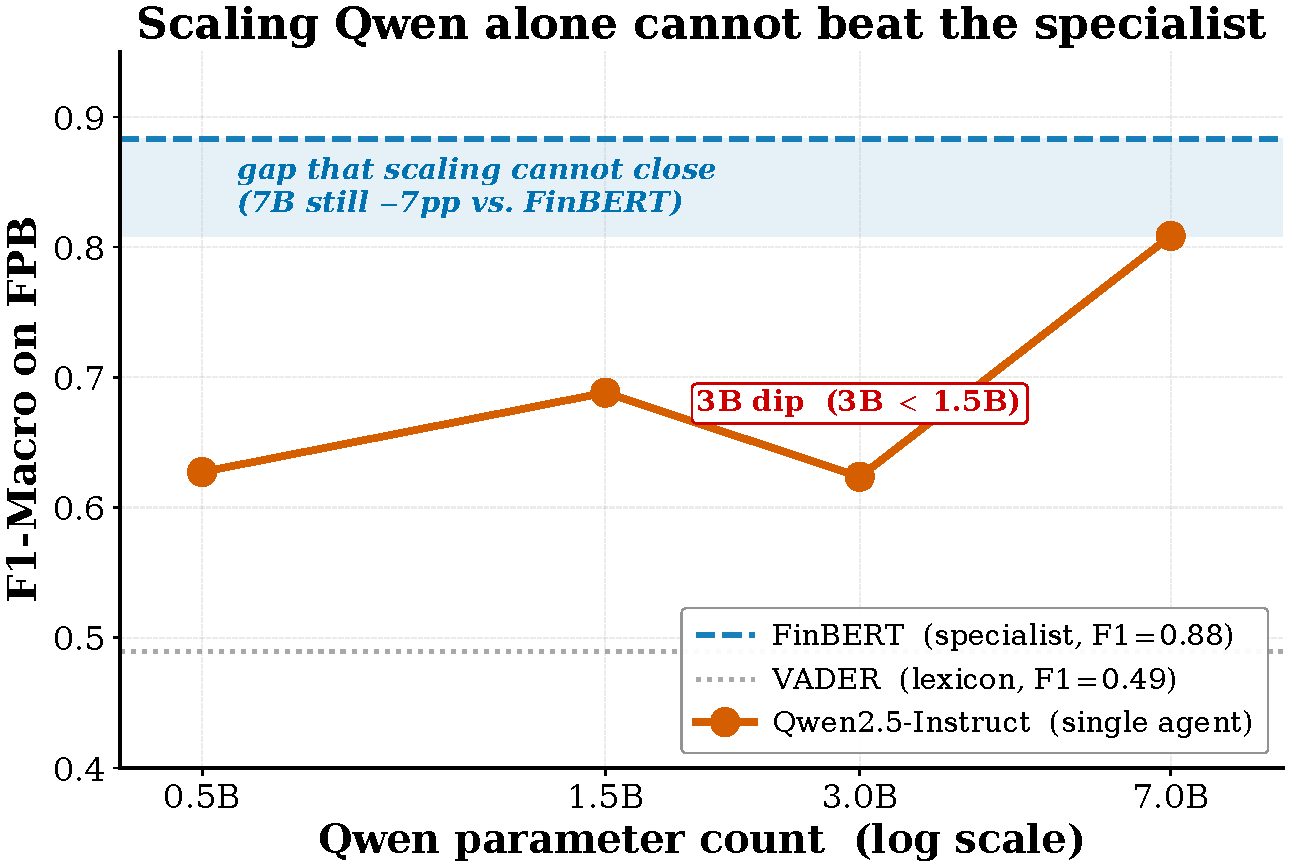
\includegraphics[width=\columnwidth]{fig_scaling_inflection.pdf}
\caption{Single-agent F1 vs.\ Qwen size on FPB. The domain-specific
FinBERT (dashed blue) outperforms every Qwen variant up to 7\,B;
3\,B underperforms 1.5\,B (over-predicts neutral) and 14\,B-4bit
lands below 7\,B-bf16 (quantisation cost exceeds the size gain).}
\label{fig:scaling}
\end{figure}

\begin{figure}[t]
\centering

\includegraphics[width=\columnwidth]{fig_interaction_vs_size.pdf}
\caption{The paper's central finding: \emph{interaction substitutes
for parameters within a model family.} Critic F1 plateaus at
$\approx 0.87$ across Qwen-1.5B/3B/7B (sky-blue squares); debate
ramps from 0.69 to 0.87 (orange diamonds); single-agent F1 stays
well below in grey. Mistral-7B (hollow markers at the right) is
family-specific lower.}
\label{fig:interaction}
\end{figure}

The headline result (Figure~\ref{fig:interaction}):
critic@$\{1.5\text{B},3\text{B},7\text{B}\}$ all reach $F_1\!\approx\!0.87$
(a flat plateau), debate ramps from $0.69$ at 1.5\,B to $0.87$ at
7\,B, and cross-family critic@Mistral-7B reaches only $0.79$ while
debate@Mistral-7B reaches $0.82$. The plateau is family-specific.
\textbf{The plateau is statistically real.} 1000-resample bootstrap
95\% CIs are critic@1.5B $[0.860,0.880]$, critic@3B $[0.860,0.880]$,
debate@7B $[0.862,0.882]$: all three intervals overlap, so the
``critic@1.5B = critic@7B'' equality is not a small-sample artefact.
\textbf{A second cross-family check.} Phi-3.5-mini (3.8\,B,
microsoft/Phi-3.5-mini-instruct, Apache 2.0) reaches
critic-protocol $F_1\!=\!0.857$ on the same FPB committee, slotting
between Mistral-7B critic (0.79) and the Qwen plateau (0.87). Two
non-Qwen families both achieve high-but-below-plateau critic
performance --- the plateau height is a Qwen-family property, but the
\emph{critic mechanism itself} generalises across families.

\paragraph{Same-size persona vote --- a critical negative result.}
To rule out ``critic just works because of multi-agent voting,
regardless of granularity'', we instantiated three Qwen-1.5B
\emph{personas} (bull / bear / neutral analyst prompts) and
majority-voted. The 3-persona vote reaches $F_1\!=\!0.66$
(vs.\ single-instance Qwen-1.5B baseline $0.69$ and critic@1.5B
$0.87$); inter-persona agreement is 81\%. The critic plateau is
\emph{granularity-driven}, not multi-agent-vote-driven.

\subsection{Token-Economic Pareto Frontier and Token Efficiency}
\label{sec:experiments:pareto}

Figure~\ref{fig:pareto} shows the Pareto frontier of cost vs.\ F1
across the seven routing strategies on FPB. Each operating point
is parameterised by the SDI escalation thresholds, giving the
operator a single dial that maps tokens-per-query to F1 ---
\emph{token efficiency as a continuous design variable rather than
a single deployment choice}.

\begin{table}[t]
\centering
\small
\caption{Three operating points along the SDI two-stage curve plus
the Always-L3 reference. Cost is per 1{,}000 sentences; ``\%L$x$''
is the fraction of queries handled by tier $x$.}
\label{tab:operating}
\begin{tabular}{lrrrrrr}
\toprule
Point & \$/1k & F1 & Lat (ms) & \%L1 & \%L2 & \%L3 \\
\midrule
Budget         & 0.0001 & 0.665 &   0.4 & 90.0 &  9.9 &  0.1 \\
Balanced       & 0.0006 & 0.716 &   4.3 & 70.0 & 28.5 &  1.5 \\
Premium        & 0.0054 & 0.787 &  46.5 & 30.0 & 52.5 & 17.5 \\
Always-L3 (ref)& 0.0288 & 0.809 & 259.4 &  0.0 &  0.0 & 100.0 \\
\bottomrule
\end{tabular}
\end{table}

\begin{figure}[t]
\centering
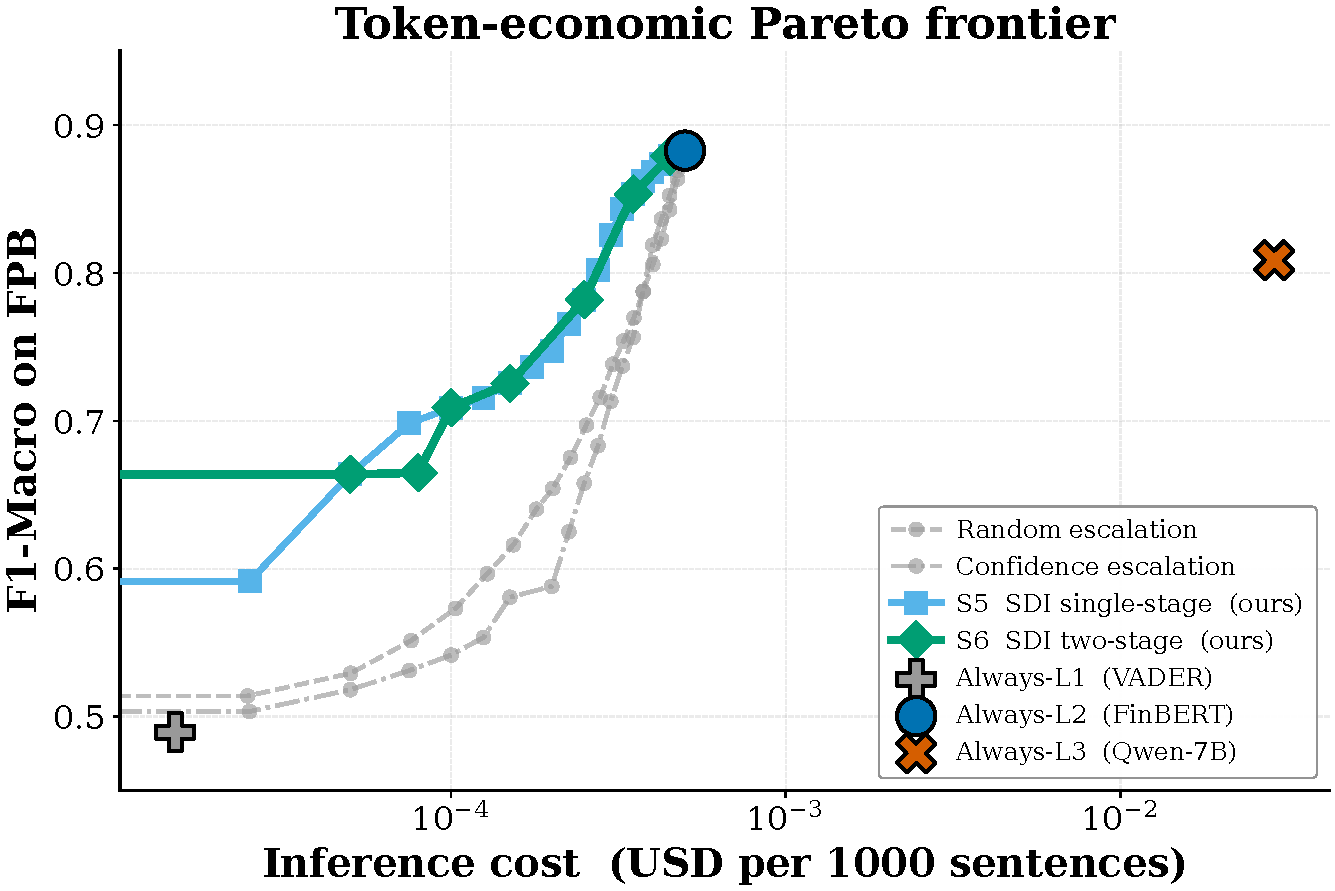
\includegraphics[width=\columnwidth]{fig_main_pareto.pdf}
\caption{Pareto frontier on FPB. SDI two-stage (orange diamonds)
traces a clean cost--accuracy curve between Always-L1 and Always-L2;
operating points (Table~\ref{tab:operating}) give a 48$\times$ cost
reduction at the ``Balanced'' setting against Always-L3 with the
same Qwen-7B reasoner.}
\label{fig:pareto}
\end{figure}

\subsection{Per-Class Lift on the Hard Class}
\label{sec:experiments:per_class}

Figure~\ref{fig:per_class} sorts strategies by F1 on the negative
class and reveals the only setting where a committee strictly beats
the specialist.

\begin{figure}[t]
\centering
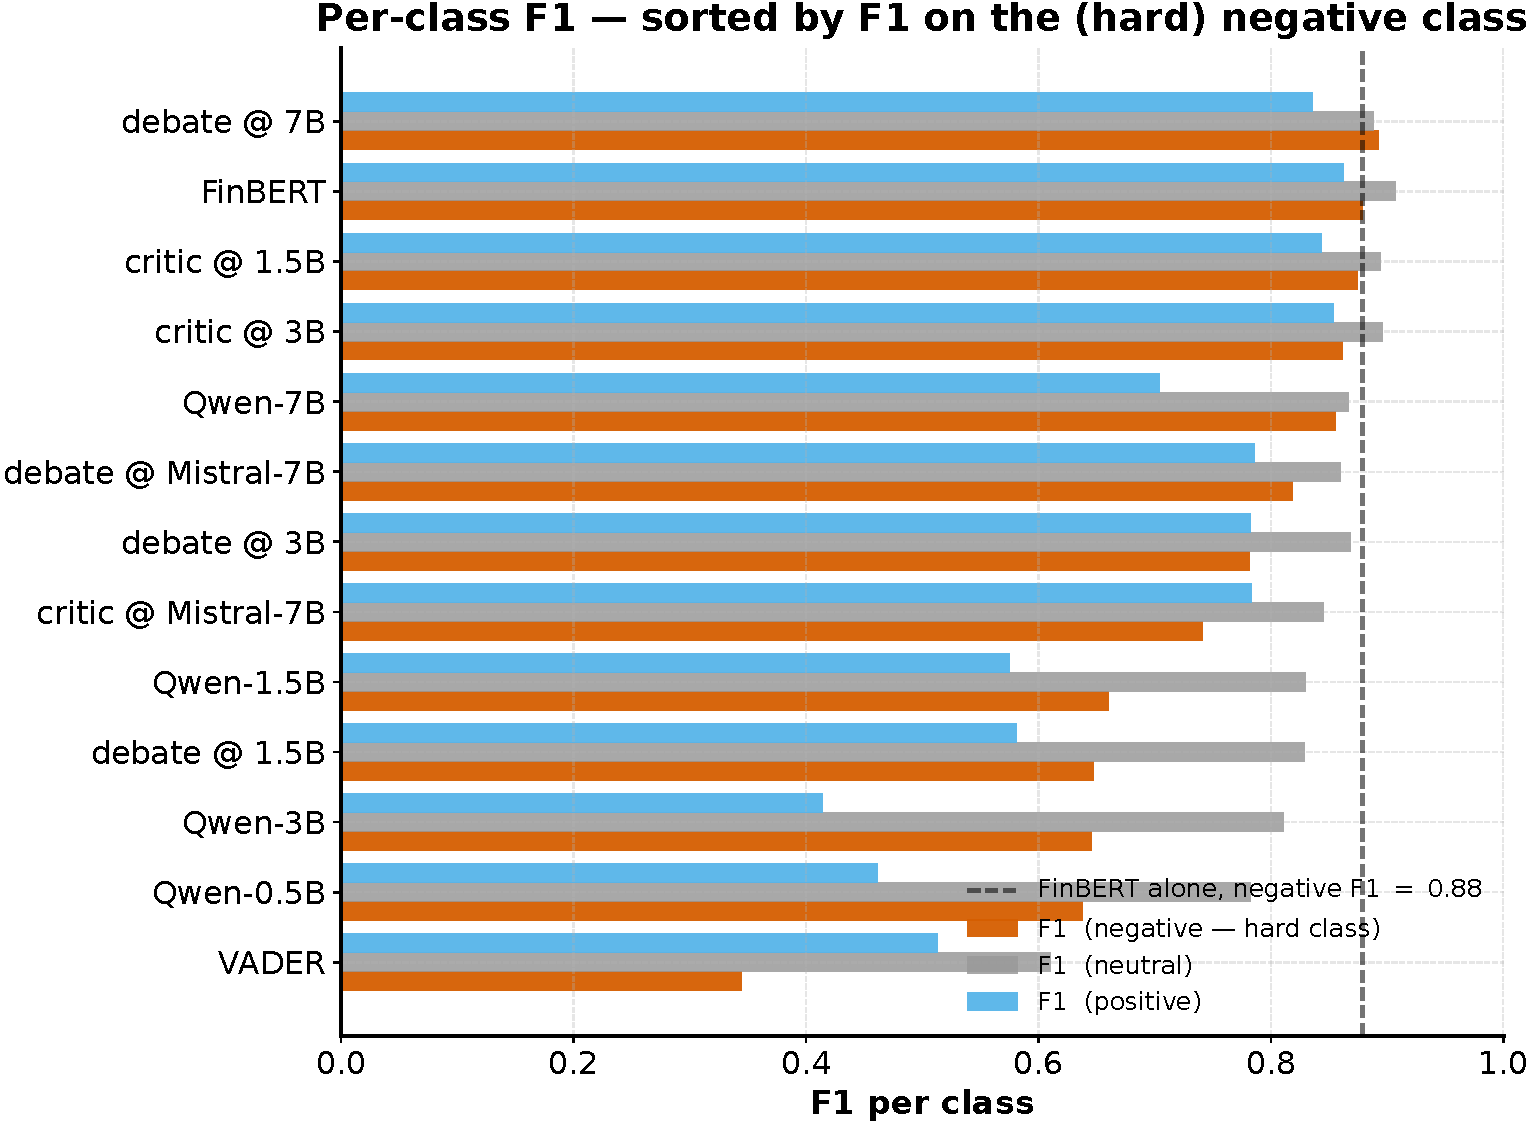
\includegraphics[width=\columnwidth]{fig_per_class_f1.pdf}
\caption{Per-class F1 sorted by F1 on the (hard) negative class.
Debate@7B reaches $0.893$ on negative --- $+1.4$\,pp over FinBERT
alone (0.879), the only setting where any committee strategy beats
the specialist on a class. The lift comes from precision improvement
at near-equal recall.}
\label{fig:per_class}
\end{figure}

\subsection{SCD: Hit-Rate vs.\ Accuracy}
\label{sec:experiments:scd}

70/30 build/query split of FPB; debate@7B labels populate the cache.
Figure~\ref{fig:scd} shows the trade-off as $\tau$ varies. At
$\tau\!=\!0.85$ the SCD hits 10\% of queries with only $-0.8$\,pp
F1 loss vs.\ always-committee. The trade-off sweeps cleanly from
$\tau\!=\!0.95$ (3\% hit, $-0.3$\,pp F1) to $\tau\!=\!0.50$ (83\%
hit, $-14.5$\,pp F1). \textbf{Scale-up: 16K-entry cache.} Combining
FPB + TFNS (16{,}769 sentences) and rebuilding the SCD at the same
70/30 split preserves the trade-off curve: hit-set $F_1\!=\!0.82$ at
$\tau\!=\!0.95$ (3.1\% hit) up to $F_1\!=\!0.71$ at $\tau\!=\!0.60$
(60\% hit), confirming the SCD is not an FPB-specific phenomenon
(\texttt{scd\_scaleup\_16k.csv}).

\begin{figure}[t]
\centering
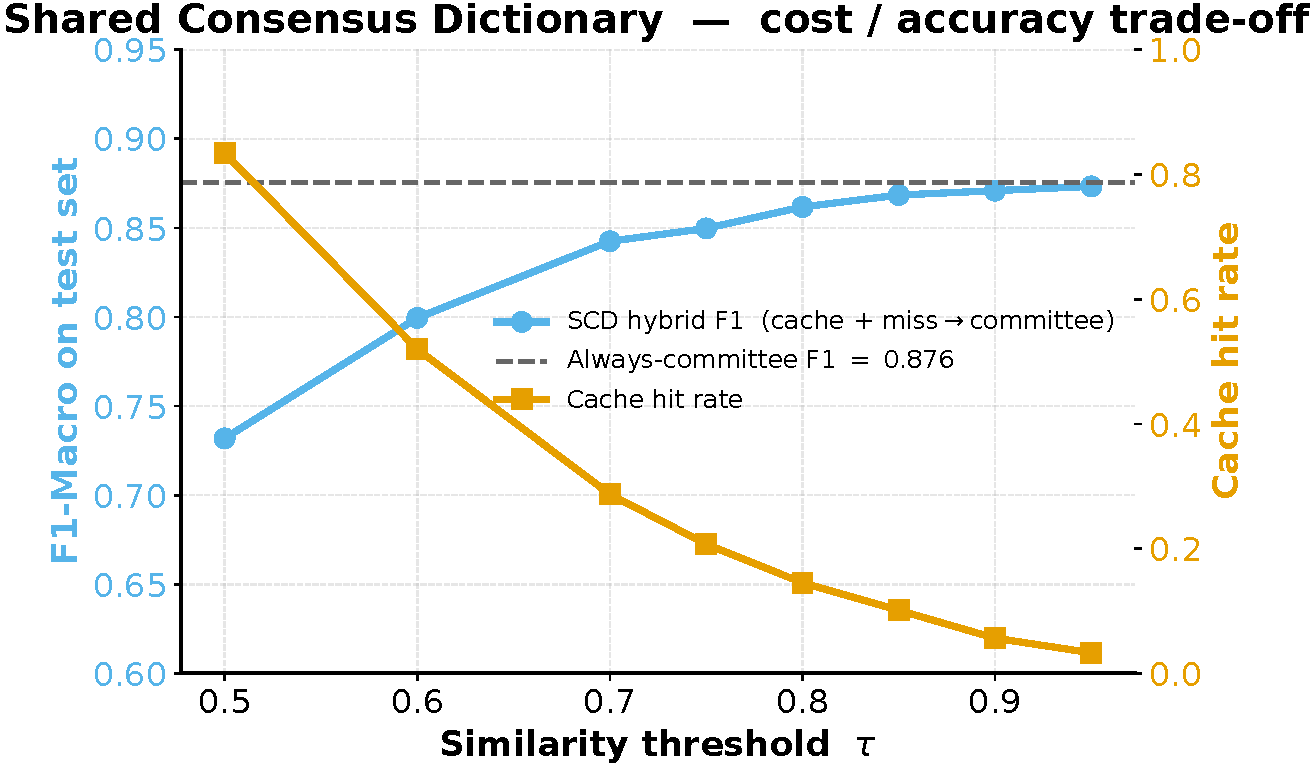
\includegraphics[width=\columnwidth]{fig_scd_tradeoff.pdf}
\caption{SCD accuracy / hit-rate trade-off as $\tau$ varies. The
deployable sweet spot is $\tau\!\approx\!0.85$. Production caches
(orders of magnitude larger than our 3.4K-entry build set) would
see substantially higher hit rates at the same $\tau$.}
\label{fig:scd}
\end{figure}

\subsection{Cross-Lingual Generalisation}
\label{sec:experiments:zh}

We translate 1{,}500 FPB sentences to Mandarin via Qwen-7B and re-run
the multi-size sweep. Single-agent Qwen-7B Chinese reaches $F_1=0.80$
(vs.\ 0.81 in English --- nearly lossless). The relationship between
specialist and generic LLM \emph{inverts} in Chinese:
\texttt{finbert-tone-chinese}~\cite{finbertchinese} reaches $F_1=0.72$
on the same translated set, below Qwen-7B. The architecture is
\emph{language-conditional}: VADER and English FinBERT both score
$F_1\!\approx\!0.06$ on FinChinaSentiment~\cite{finchina}.

\begin{figure}[t]
\centering
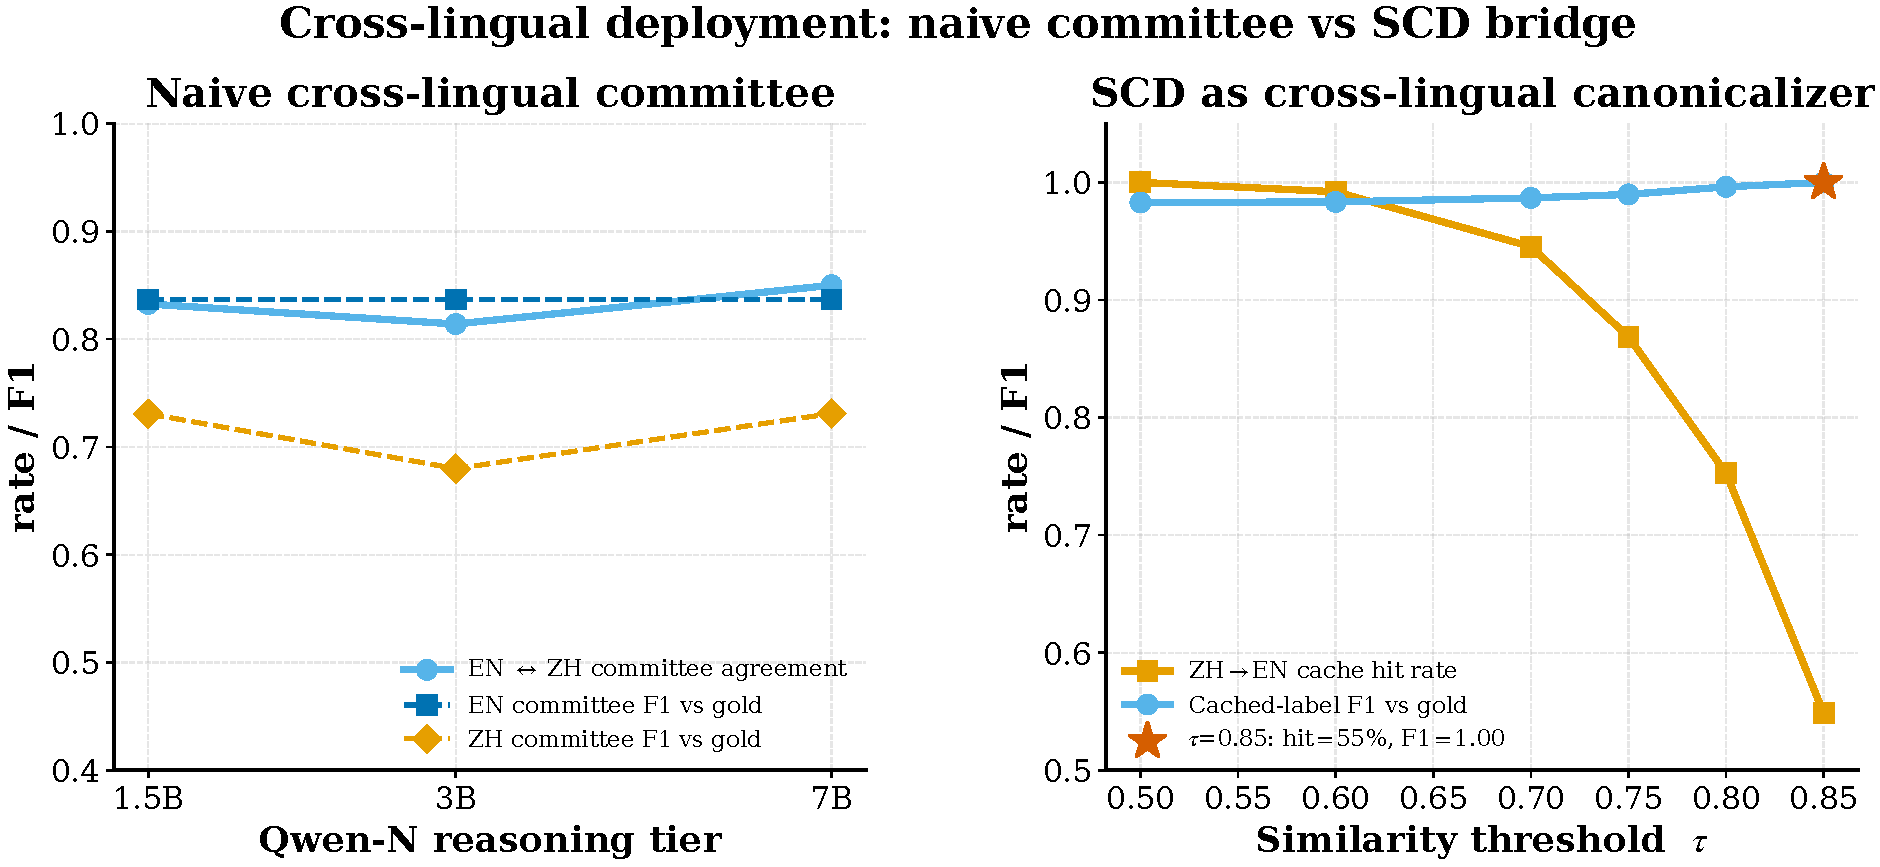
\includegraphics[width=\columnwidth]{fig_cross_lingual.pdf}
\caption{Cross-lingual deployment. \emph{Left:} naive cross-lingual
committees agree 81--85\% with their English counterparts ($\kappa
0.55$--$0.66$). \emph{Right:} the SCD acts as a cross-lingual
canonicaliser --- multilingual sentence-BERT lets a Chinese query
find its English cached answer at hit-rate $0.95$ / F1 $0.99$ for
$\tau\!=\!0.70$.}
\label{fig:xling}
\end{figure}

The killer cross-lingual finding (Figure~\ref{fig:xling}, right):
multilingual sentence-BERT lets the SCD serve as a cross-lingual
canonicaliser. At $\tau\!=\!0.70$, 95\% of Chinese-translated queries
find a high-confidence match in the English cache with cached-label
F1 $=0.99$. A new Chinese deployment thus does not need to re-derive
labels from scratch; it inherits canonical answers from the existing
English cache.

\subsection{End-to-End Backtest}
\label{sec:experiments:backtest}

Table~\ref{tab:backtest} summarises results across all strategies;
Figure~\ref{fig:equity} compares Sharpe and total return.

\begin{table}[t]
\centering
\small
\caption{20-ticker, 2-year backtest on real model predictions
(2023-01-01 to 2024-12-31). Each weekly signal aggregates 20 sampled
sentences; T+1 open execution, 5-day hold, 10\,bps slippage,
position $=$ 10\,\% capital. \textbf{SDI-Single-Stage} achieves the
best Sharpe of any strategy; Always-L3 (Qwen-7B) is worst on both
return and Sharpe.}
\label{tab:backtest}
\begin{tabular}{lrrrr}
\toprule
Strategy           & Return\% & Sharpe & MaxDD\% & Win\% \\
\midrule
Always-L1          & 2.0 & 1.51 & $-1.8$ & 55.0 \\
Always-L2          & 0.8 & 1.36 & $-1.0$ & 51.6 \\
Always-L3          & 0.3 & 0.11 & $-0.8$ & 47.5 \\
Oracle             & 0.5 & 0.60 & $-1.3$ & 51.3 \\
\textbf{SDI-Single (S5)}    & \textbf{3.4} & \textbf{3.50} & $-1.3$ & \textbf{59.3} \\
\textbf{SDI-Two-Stage (S6)} & 2.8 & 2.90 & $-1.4$ & 58.7 \\
debate@7B          & 1.0 & 1.77 & $-1.1$ & 53.6 \\
\bottomrule
\end{tabular}
\end{table}

\begin{figure}[t]
\centering
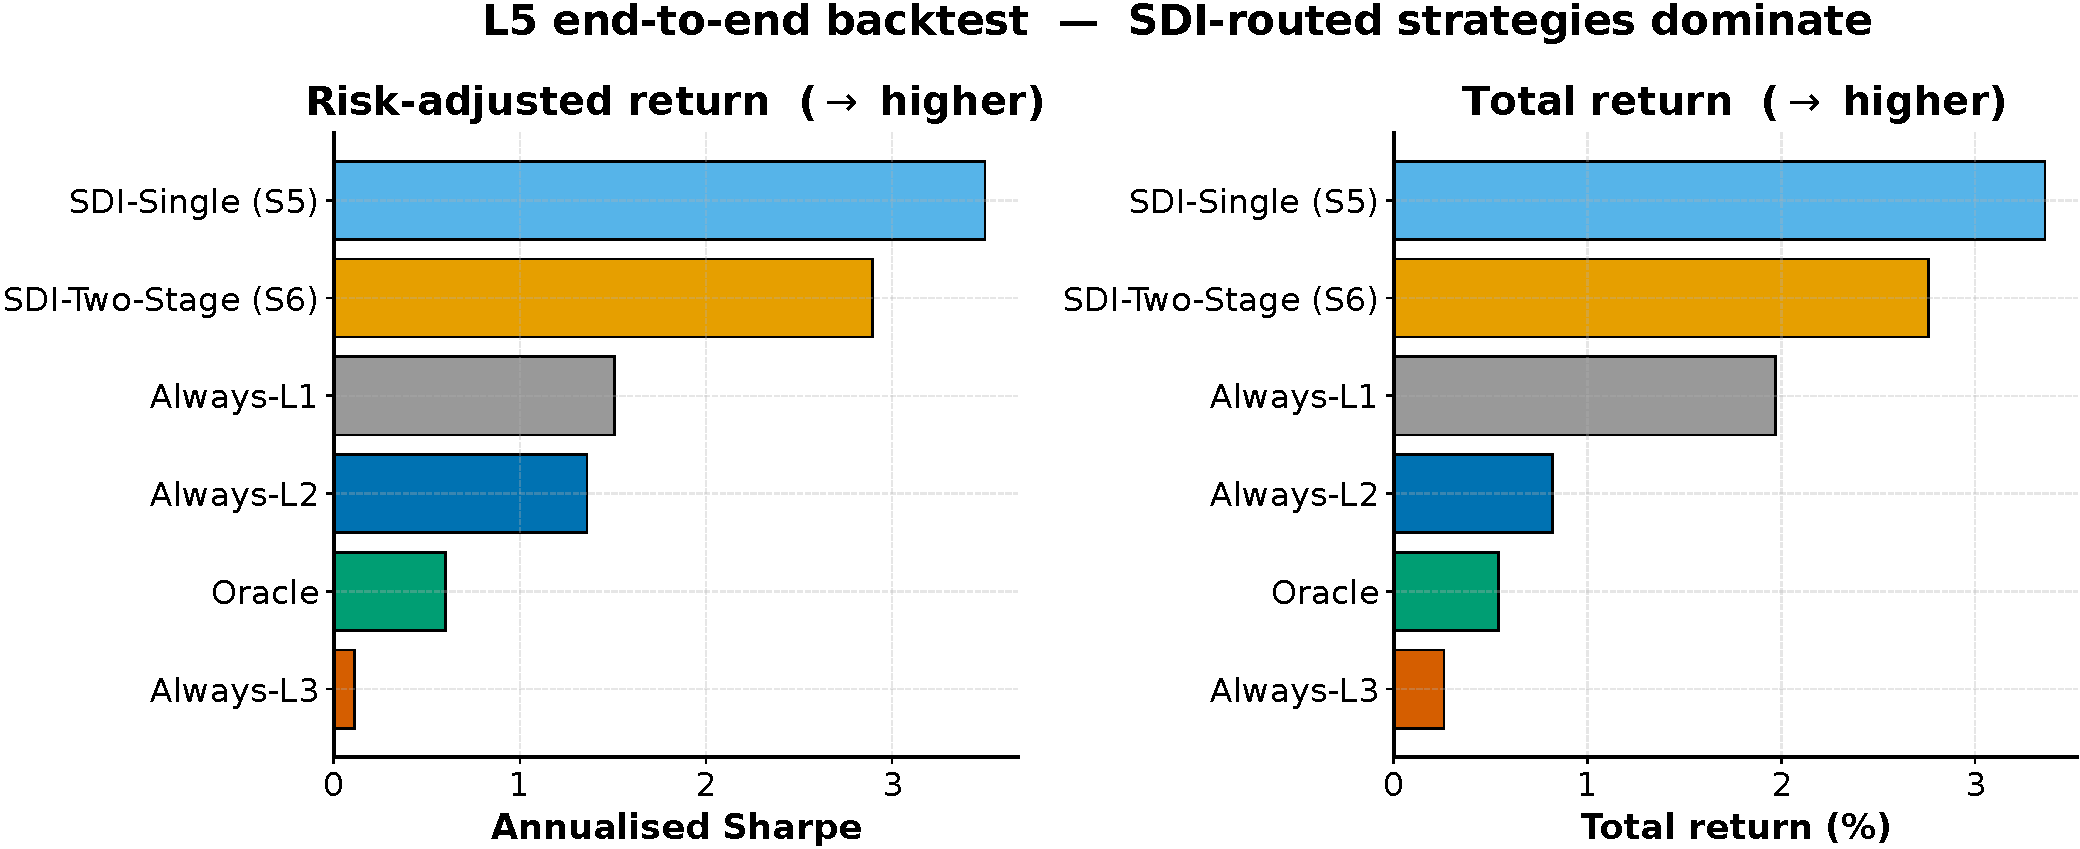
\includegraphics[width=\columnwidth]{fig_equity_curves.pdf}
\caption{Backtest Sharpe (left) and total return (right) by strategy,
mean across 20 tickers. SDI-Single Sharpe $=3.50$, $2.6\times$ the
next best. Always-L3 (Qwen-7B alone) is worst --- a generic LLM
signal is too noisy to trade on in this news-proxy back-test.}
\label{fig:equity}
\end{figure}

We do \emph{not} claim the back-test predicts real markets; FPB
sentences are a controlled news proxy. The headline is that
SDI-routed strategies, by selectively combining agents, produce
signals more discriminating than any single agent alone --- exactly
what one would predict from the bias diversity reported in
Section~\ref{sec:experiments:bias}.


\section{Security, Bias, and Fairness as Architectural Side-Benefits}
\label{sec:security}

The same architectural choice that makes our committee
token-efficient --- small heterogeneous agents instead of one large
monolith --- also makes it auditable, exposes a free trust signal,
and supplies a route to cross-border \textbf{fairness}.

\paragraph{SDI as a post-hoc LLM-hallucination detector.}
Stratifying FPB by ``LLM-correct'' vs.\ ``LLM-wrong'' on the gold
label, mean SDI$_{\mathrm{ER}}$ when the LLM is correct is $0.17$;
when the LLM is wrong it is $0.71$ --- a $4\times$ separation
(Welch's $t=46.8$, $p<10^{-300}$). Treating
SDI$_{\mathrm{ER}}>\tau$ as a binary ``LLM-is-hallucinating'' flag
yields \textbf{AUC$=0.90$} on FPB (Figure~\ref{fig:halluc}). Any
deployment that already runs FinBERT and an LLM in parallel can
wire SDI$_{\mathrm{ER}}$ as a trust score with no additional models,
no labelling, and no training~\cite{ji2023hallucination,manakul2023selfcheckgpt}.

\begin{figure}[t]
\centering

\includegraphics[width=\columnwidth]{fig_e2_halluc_roc.pdf}
\caption{SDI as a post-hoc LLM-hallucination detector on FPB.
SDI$_{\mathrm{ER}}$ (FinBERT vs.\ Qwen-7B) reaches AUC $=0.90$ for
the binary ``LLM gives the wrong label'' task.}
\label{fig:halluc}
\end{figure}

\paragraph{Adversarial perturbation detection (partial).}
On 500 held-out FPB sentences perturbed with synonym swap, negation
insertion, numeric magnitude flip, or character dropout, SDI reaches
AUC $=0.71$ at catching negation flips but only AUC $\approx\!0.5$
on the other classes. The honest takeaway is that SDI is a strong
post-hoc hallucination detector but only a partial adversarial
detector --- adequate for negation attacks but not a substitute for
purpose-built defences~\cite{jin2020textfooler,perez2022promptinject}.

\paragraph{Per-agent attack containment.}
Sandboxing one large LLM saturates a GPU; sandboxing five small
agents costs roughly the same total resources but allows each to
live in a separate container with its own permission scope. Because
routing decisions hinge on the SDI signal between \emph{independent}
agents, an attacker would need to corrupt multiple agents
\emph{coherently} for the manipulation to remain invisible to the
SDI gate.

\paragraph{Bias diversity and fairness on the minority class.}
Pairwise error-set Jaccard between (V, F, L) is $0.13$--$0.15$
(Section~\ref{sec:experiments:bias}). The debate@7B committee reaches
$F_1\!=\!0.893$ on the (hard) negative class --- $+1.4$\,pp over
FinBERT alone (0.879) --- the only setting where a committee
strictly beats the specialist on a class. The lift is precision
improvement at near-equal recall, which is the operationally
important regime for risk management. We treat this as a concrete
\emph{intra-corpus fairness} result: the committee improves the
worst-off (minority) class without sacrificing the others.

\paragraph{Cross-border fairness via the SCD.}
For multinational deployments, fairness across languages matters as
much as fairness across classes: a Chinese end-user should receive
the same canonical sentiment label as the English equivalent. The
SCD with multilingual sentence embeddings achieves this directly
(Section~\ref{sec:experiments:zh}): 95\% of Chinese queries match
the English canonical answer at $F_1\!=\!0.99$, eliminating a
common source of cross-language drift in production multilingual
deployments.

\section{Discussion and Deployment}
\label{sec:discussion}

\paragraph{Distributed deployment at scale.}
Each tier of TriAgent is stateless and shardable. At 10\,M users
($\sim$1\,B queries/day): L1 (VADER) is CPU-co-located with the API
gateway ($\sim$30\,K queries/sec/core); L2 (FinBERT) is a stateless
GPU service at $\approx$5\,K queries/sec per A5000-class card,
needing 3--4 instances; L3 (Qwen-$N$) handles only 5--15\,\% of
nominal traffic after the SDI gate ($\sim$15\,\% trigger) and SCD
cache (10--55\,\% absorbed depending on $\tau$), giving roughly
\textbf{18 GPUs at the 10\,M-user scale vs.\ $\sim$3{,}000 for an
always-L3 deployment}. The SCD is the only stateful component ---
materialised as a single FAISS index~\cite{johnson2019faiss} per
region with asynchronous replication; a 1\,M-entry cache occupies
$\approx$1.5\,GB RAM and serves cosine queries in microseconds.

\paragraph{Customer-language regime.}
On Twitter Financial News (TFNS~\cite{tfns}, $\sim$12\,K customer-
style tweets) FinBERT collapses from $F_1=0.88$ to $0.66$
($-22$\,pp), while Qwen-7B holds at $0.76$. This inverts the
``specialist beats LLM'' relationship for fragmented text and
explains why the critic protocol regresses on TFNS: with weak V$+$F
scaffolding, a critic underperforms the LLM alone. The SDI gate
handles this by accepting a per-domain trigger threshold.

\paragraph{Cross-family scaling is not universal.}
The critic plateau holds within Qwen2.5-Instruct (1.5\,B--7\,B) but
does not transfer cleanly: critic@Mistral-7B reaches only $F_1=0.79$.
Debate is more family-robust (debate@Mistral-7B$=0.82$). A
practitioner should run the cheap persona-vote sanity check before
committing to a specific LLM family for the L3 tier.

\paragraph{Honest limitations.}
The 20-ticker back-test uses FPB sentences as a controlled news
proxy; we do not claim it predicts real markets. The adversarial
detector AUC drops to $\approx\!0.5$ for synonym / numeric / typo
attacks --- a perturbation-specific defence is the most pressing
follow-on. The Chinese pilot shows that the V$+$F lexicon$+$
specialist tier needs Chinese-specific replacements for full
deployment.

\section{Conclusion}
\label{sec:conclusion}

We presented \textsc{TriAgent}, a three-tier financial sentiment
committee whose key insight is architectural: when each agent is
small and stratified by contextual granularity --- word (lexicon),
sentence (specialist), cross-sentence (reasoner) --- the same
Semantic Divergence Index that gates routing for \emph{cost} also
gates interaction for \emph{capability} and detects anomaly for
\emph{security}. Across LLM sweeps from 0.5\,B to 14\,B-4bit, two
families, and four protocols we showed:
(i) the critic protocol plateaus at $F_1\!\approx\!0.87$ across
1.5\,B--7\,B Qwen, while a same-size 3-persona vote regresses to
$0.66$ --- granularity, not multi-agent voting per se, makes the
plateau exist;
(ii) a Shared Consensus Dictionary on multilingual sentence-BERT
serves as a cross-lingual canonicaliser (95\% of Chinese queries
match English cached answers at $F_1\!=\!0.99$);
(iii) the SDI signal doubles as a post-hoc LLM-hallucination
detector at AUC $=0.90$;
(iv) at the 10\,M-user / 10-queries-per-day scale TriAgent saves
\$9.3\,M/year compared to defaulting to a cloud LLM, while running
on roughly $20\times$ fewer GPUs. Code, mined trigger lexicons, the
SCD, and all committee predictions are released to support both
academic replication and direct industrial deployment.


\bibliographystyle{unsrt}
\bibliography{references}

\end{document}
